\documentclass[a4paper,11pt,exos]{nsi} % COMPILE WITH DRAFT


\pagestyle{empty}
\begin{document}

%Exercice 1E12


\subsection*{NOM, Prénom : \dotfill} 

\classe{\premiere spé}
\titre{Ceinture bleue 01}
\maketitle

\begin{exercice}[ : Trouver l'équation d'une parabole]
    Quelle est l'expression de la fonction polynomiale $f$ du second degré qui s'annule en $x=-4$ et en $x=1$ et dont la parabole passe par le point de coordonnées $(2;-18)$ ?\\
    Donner la forme développée de $f$.\\
    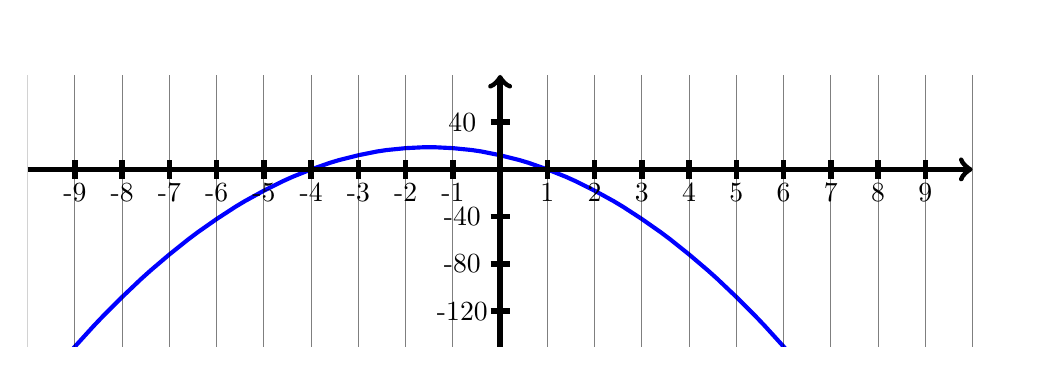
\begin{tikzpicture}[baseline,scale = 0.6]

        \tikzset{
          point/.style={
            thick,
            draw,
            cross out,
            inner sep=0pt,
            minimum width=5pt,
            minimum height=5pt,
          },
        }
        \clip (-10,-3.75) rectangle (11,3);
            
        \draw[color={blue},line width = 1.5] (-10,-4.95)--(-9.8,-4.7)--(-9.6,-4.45)--(-9.4,-4.21)--(-9.2,-3.98)--(-9,-3.75)--(-8.8,-3.53)--(-8.6,-3.31)--(-8.4,-3.1)--(-8.2,-2.9)--(-8,-2.7)--(-7.8,-2.51)--(-7.6,-2.32)--(-7.4,-2.14)--(-7.2,-1.97)--(-7,-1.8)--(-6.8,-1.64)--(-6.6,-1.48)--(-6.4,-1.33)--(-6.2,-1.19)--(-6,-1.05)--(-5.8,-0.92)--(-5.6,-0.79)--(-5.4,-0.67)--(-5.2,-0.56)--(-5,-0.45)--(-4.8,-0.35)--(-4.6,-0.25)--(-4.4,-0.16)--(-4.2,-0.08)--(-4,0)--(-3.8,0.07)--(-3.6,0.14)--(-3.4,0.2)--(-3.2,0.25)--(-3,0.3)--(-2.8,0.34)--(-2.6,0.38)--(-2.4,0.41)--(-2.2,0.43)--(-2,0.45)--(-1.8,0.46)--(-1.6,0.47)--(-1.4,0.47)--(-1.2,0.46)--(-1,0.45)--(-0.8,0.43)--(-0.6,0.41)--(-0.4,0.38)--(-0.2,0.34)--(0,0.3)--(0.2,0.25)--(0.4,0.2)--(0.6,0.14)--(0.8,0.07)--(1,0)--(1.2,-0.08)--(1.4,-0.16)--(1.6,-0.25)--(1.8,-0.35)--(2,-0.45)--(2.2,-0.56)--(2.4,-0.67)--(2.6,-0.79)--(2.8,-0.92)--(3,-1.05)--(3.2,-1.19)--(3.4,-1.33)--(3.6,-1.48)--(3.8,-1.64)--(4,-1.8)--(4.2,-1.97)--(4.4,-2.14)--(4.6,-2.32)--(4.8,-2.51)--(5,-2.7)--(5.2,-2.9)--(5.4,-3.1)--(5.6,-3.31)--(5.8,-3.53)--(6,-3.75)--(6.2,-3.98)--(6.4,-4.21)--(6.6,-4.45)--(6.8,-4.7)--(7,-4.95);
        \draw[color={blue},line width = 1.5] ;
        \draw[color={blue},line width = 1.5] ;
        \draw[color={blue},line width = 1.5] ;
        \draw[color={blue},line width = 1.5] ;
        \draw[color={blue},line width = 1.5] ;
        \draw[color={blue},line width = 1.5] ;
        \draw[color={blue},line width = 1.5] ;
        \draw[color={blue},line width = 1.5] ;
        \draw[color={blue},line width = 1.5] ;
        \draw[color={blue},line width = 1.5] ;
        \draw[color={blue},line width = 1.5] ;
        \draw[color={blue},line width = 1.5] ;
        \draw[color={blue},line width = 1.5] ;
        \draw[color={blue},line width = 1.5] ;
        \draw[color={blue},line width = 1.5] ;
        
        \draw[color ={black},line width = 2,->] (-10,0)--(10,0);
        \draw[color ={black},line width = 2,->] (0,-5)--(0,2);
        \draw[color ={black},opacity = 0.5] (1,-5)--(1,2);
        \draw[color ={black},opacity = 0.5] (2,-5)--(2,2);
        \draw[color ={black},opacity = 0.5] (3,-5)--(3,2);
        \draw[color ={black},opacity = 0.5] (4,-5)--(4,2);
        \draw[color ={black},opacity = 0.5] (5,-5)--(5,2);
        \draw[color ={black},opacity = 0.5] (6,-5)--(6,2);
        \draw[color ={black},opacity = 0.5] (7,-5)--(7,2);
        \draw[color ={black},opacity = 0.5] (8,-5)--(8,2);
        \draw[color ={black},opacity = 0.5] (9,-5)--(9,2);
        \draw[color ={black},opacity = 0.5] (10,-5)--(10,2);
        \draw[color ={black},opacity = 0.5] (-1,-5)--(-1,2);
        \draw[color ={black},opacity = 0.5] (-2,-5)--(-2,2);
        \draw[color ={black},opacity = 0.5] (-3,-5)--(-3,2);
        \draw[color ={black},opacity = 0.5] (-4,-5)--(-4,2);
        \draw[color ={black},opacity = 0.5] (-5,-5)--(-5,2);
        \draw[color ={black},opacity = 0.5] (-6,-5)--(-6,2);
        \draw[color ={black},opacity = 0.5] (-7,-5)--(-7,2);
        \draw[color ={black},opacity = 0.5] (-8,-5)--(-8,2);
        \draw[color ={black},opacity = 0.5] (-9,-5)--(-9,2);
        \draw[color ={black},opacity = 0.5] (-10,-5)--(-10,2);
        \draw[color ={black},line width = 2] (1,-0.2)--(1,0.2);
        \draw[color ={black},line width = 2] (2,-0.2)--(2,0.2);
        \draw[color ={black},line width = 2] (3,-0.2)--(3,0.2);
        \draw[color ={black},line width = 2] (4,-0.2)--(4,0.2);
        \draw[color ={black},line width = 2] (5,-0.2)--(5,0.2);
        \draw[color ={black},line width = 2] (6,-0.2)--(6,0.2);
        \draw[color ={black},line width = 2] (7,-0.2)--(7,0.2);
        \draw[color ={black},line width = 2] (8,-0.2)--(8,0.2);
        \draw[color ={black},line width = 2] (9,-0.2)--(9,0.2);
        \draw[color ={black},line width = 2] (-1,-0.2)--(-1,0.2);
        \draw[color ={black},line width = 2] (-2,-0.2)--(-2,0.2);
        \draw[color ={black},line width = 2] (-3,-0.2)--(-3,0.2);
        \draw[color ={black},line width = 2] (-4,-0.2)--(-4,0.2);
        \draw[color ={black},line width = 2] (-5,-0.2)--(-5,0.2);
        \draw[color ={black},line width = 2] (-6,-0.2)--(-6,0.2);
        \draw[color ={black},line width = 2] (-7,-0.2)--(-7,0.2);
        \draw[color ={black},line width = 2] (-8,-0.2)--(-8,0.2);
        \draw[color ={black},line width = 2] (-9,-0.2)--(-9,0.2);
        \draw[color ={black},line width = 2] (-0.2,1)--(0.2,1);
        \draw[color ={black},line width = 2] (-0.2,-1)--(0.2,-1);
        \draw[color ={black},line width = 2] (-0.2,-2)--(0.2,-2);
        \draw[color ={black},line width = 2] (-0.2,-3)--(0.2,-3);
        \draw[color ={black},line width = 2] (-0.2,-4)--(0.2,-4);
        \draw [color={black},fill opacity = 1] (1,-0.5) node[anchor = center,scale=1] {1};
        \draw [color={black},fill opacity = 1] (2,-0.5) node[anchor = center,scale=1] {2};
        \draw [color={black},fill opacity = 1] (3,-0.5) node[anchor = center,scale=1] {3};
        \draw [color={black},fill opacity = 1] (4,-0.5) node[anchor = center,scale=1] {4};
        \draw [color={black},fill opacity = 1] (5,-0.5) node[anchor = center,scale=1] {5};
        \draw [color={black},fill opacity = 1] (6,-0.5) node[anchor = center,scale=1] {6};
        \draw [color={black},fill opacity = 1] (7,-0.5) node[anchor = center,scale=1] {7};
        \draw [color={black},fill opacity = 1] (8,-0.5) node[anchor = center,scale=1] {8};
        \draw [color={black},fill opacity = 1] (9,-0.5) node[anchor = center,scale=1] {9};
        \draw [color={black},fill opacity = 1] (-1,-0.5) node[anchor = center,scale=1] {-1};
        \draw [color={black},fill opacity = 1] (-2,-0.5) node[anchor = center,scale=1] {-2};
        \draw [color={black},fill opacity = 1] (-3,-0.5) node[anchor = center,scale=1] {-3};
        \draw [color={black},fill opacity = 1] (-4,-0.5) node[anchor = center,scale=1] {-4};
        \draw [color={black},fill opacity = 1] (-5,-0.5) node[anchor = center,scale=1] {-5};
        \draw [color={black},fill opacity = 1] (-6,-0.5) node[anchor = center,scale=1] {-6};
        \draw [color={black},fill opacity = 1] (-7,-0.5) node[anchor = center,scale=1] {-7};
        \draw [color={black},fill opacity = 1] (-8,-0.5) node[anchor = center,scale=1] {-8};
        \draw [color={black},fill opacity = 1] (-9,-0.5) node[anchor = center,scale=1] {-9};
        \draw [color={black},fill opacity = 1] (-0.8,1) node[anchor = center,scale=1] {40};
        \draw [color={black},fill opacity = 1] (-0.8,-1) node[anchor = center,scale=1] {-40};
        \draw [color={black},fill opacity = 1] (-0.8,-2) node[anchor = center,scale=1] {-80};
        \draw [color={black},fill opacity = 1] (-0.8,-3) node[anchor = center,scale=1] {-120};
        \draw [color={black},fill opacity = 1] (-0.8,-4) node[anchor = center,scale=1] {-160};
    
    \end{tikzpicture}\\
\end{exercice}


Comme $-4$ et $1$ sont les deux solutions de l'équation $f(x)=0$, on peut factoriser $f(x)$ :\\$f(x)=a(x+4)(x-1)$.\\Comme $f(2)=-18$, on en déduit que $-18=a(2+4)(2-1)$ d'où $a=-18\div 6=-3$.\\On obtient ainsi $f(x)=-3(x+4)(x-1)$ ou en développant $f(x)=-3x^2 -9x  +12$

\end{document}